\chapter{The Chain}\label{chapter:chain}

In the last chapter, we discussed the necessity for blocks as a mechanism to enforce \emph{periods of silence} so that double spends
can be adequately separated in time.  We then linked blocks together into chains in order to ensure freshness so that an adversary cannot
retroactively bring blocks mined and withheld in the old past. However, we left the notion of ``freshness'' and block validation
undefined. In this chapter, we will fill in all the missing details of how blocks and chains are verified. By the end of this chapter,
we will have a rudimentary, yet complete and secure, blockchain protocol.

\section{The Target}

Previously, we designed the proof-of-work inequality $H(B) \leq T$ in order to create \emph{rare events} and \emph{periods of silence}
as a moderately hard version of the exponentially hard hash preimage problem. In order to prevent double spends, we needed to ensure
that blocks are spaced $\Delta$ apart. Let us now calculate the correct value of $T$ so that block production is spaced more than
$\Delta$ time apart. To do this, we need to first find out when the proof-of-work inequality holds. If we start
with a freshly generated $\ctr$ and place it into $B = s \conc \overline{x} \conc \ctr$, what is the probability that $H(B) \leq T$?
This question is not straightforward to answer, because the output of a hash function may not be uniformly distributed (see also
Problem~\ref{problem:small-hash}).

In fact, not all collision resistant hash functions are suitable for proof-of-work. We want to demand that, whenever the hash is queried with a fresh input, the output is uniformly distributed in $\{0,1\}^\kappa$. This extra assumption is known as the \emph{random oracle model} and we will return to it in Chapter~\ref{chapter:earnest1}. Using the random oracle model, we can calculate the probability that a particular nonce trial is successful:

\glsxtrnewsymbol[description={successful query probability}]{successful query probability}{$p$}\glsadd{successful query probability}
\[
  p = \Pr[H(B) \leq T] = \frac{T}{2^\kappa}
\]

During the exhaustive search of proof-of-work, if a particular hash trial $H(B)$ is found to be $H(B) \leq T$, we call that hash function query a \emph{successful query}\index{Successful query}. Otherwise, if $H(B) > T$, we call the query \emph{unsuccessful}. The expected number of queries needed until a successful query is found is $\frac{1}{p} = \frac{2^\kappa}{T}$.

As protocol designers, we need to set $T$ correctly so that blocks are produced at a rate smaller than once per $\Delta$. For this, we need to have an estimate of how fast the participating nodes on the network can compute hash queries. Let's start with some definitions. Suppose that a typical honest computer can process
\glsxtrnewsymbol[description={compute}]{compute}{$q$}\glsadd{compute}
$q \in \mathbb{N}$
computations of $H$ during every unit of time. Let us also suppose that the total number of computers mining on the network is
\glsxtrnewsymbol[description={total parties}]{total parties}{$n$}\glsadd{total parties}
$n \in \mathbb{N}$
and the adversary controls
\glsxtrnewsymbol[description={adversarial parties}]{adversarial parties}{$t$}\glsadd{adversarial parties}
$t \in \mathbb{N}$
of them. Here, we are assuming that all computers have equal processing power, but if there is some computer on the network that has more processing power, we can just think about that powerful computer as a collection of smaller, less powerful computers, each of which has $q$ computational power. The model still works out. We will call each of these computers a
\emph{party}\index{Party}.
Each mining party will roughly correspond to a node on the network, but in practice these are not necessarily the same: A single network node can correspond to multiple parties if it is a powerful computer. On the other hand, because our system is permissionless, a party may spawn multiple nodes that all share the same computational power. Additionally, even though we are saying that the adversary is in control of $t$ adversarial parties, we are still considering the situation where the adversary is a ``puppet master'' who controls every adversarial party of the network by a central ``master plan'' $\mathcal{A}$. We say that such a party controlled by the adversary is \emph{adversarial}, \emph{corrupt}, or \emph{malicious}, and we will use these terms interchangably.

The total number of hash queries that can be executed in the unit of time is $nq$.
Since all parties are simultaneously trying to get a block all the time, the expected block generation
time is $\frac{1}{pnq} = \frac{2^\kappa}{Tnq}$. If we want this value to be above $\Delta$ we must demand

\[
  \frac{2^\kappa}{Tnq} > \Delta \Rightarrow T < \frac{2^\kappa}{nq\Delta}\,.
\]

In a nutshell, the more computational power there is on the network, the larger we must make the difficulty.
Also, the larger the network delay, the larger we must make the difficulty.
We will use $f$ to denote the honest block production rate (expected blocks per unit of time),
and $\eta = \frac{1}{f}$ the expected time between two blocks being generated.
For now, we'll estimate that $f \simeq (n - t)qp$, but we will give a more
formal definition for $f$ in Chapter~\ref{chapter:earnest1}.

As the designers of the protocol, we will make some reasonable estimations for $\Delta$, $n$, $t$ and $q$.
Based on these, we will calculate the value $T$. For the time being, we will fix $T$ to be a constant
that never changes. This model is called the \emph{static difficulty model}. We'll revisit this assumption
in Chapter~\ref{chapter:economics}.

\section{The Arrow of Time}

In the previous chapter, we decided to link blocks together into a chain in order to ensure each block
has \emph{freshness} and cannot be brought back from the past. It turns out that this natural and
intuitive chain structure actually has many more nice properties than just ensuring freshness, which
we will explore over the next few chapters.

In order to be able to speak about chains more precisely,
let us introduce a bit of notation. A chain $\chain$ is a finite sequence of blocks
$\chain = (B_0, B_1, B_2, \ldots, B_{n-1})$ ordered chronologically.
The chain \emph{length} $|\chain|$ is the number of blocks in the chain.
We address these blocks by their zero-based index,
so $\chain[0]$ is the first (and oldest) block on the chain, $\chain[1]$ is the second, and so on.
The first block among a complete chain is the genesis block, so $\chain[0] = \mathcal{G}$.
We use negative indexing to address blocks from the end of the chain, so $\chain[-1]$
is the last (and most recent) block, $\chain[-2]$ is the penultimate block, and so on.
The block $\chain[-1]$ is called the \emph{tip}.
The index of a block within its chain is called the block's \emph{height},
so genesis has height $0$ and the tip has height $|\chain| - 1$.
The \emph{depth} of a block within its chain is the distance of a block
from the tip. For example, the tip has depth $1$, the block preceding the
tip has depth $2$ and so on.
It will also be useful to speak about \emph{chunks} of a chain, continuous portions
of the chain. We'll denote by $\chain[i{:}j]$ the portion of the chain starting at block
with index $i$ (inclusive) and ending at block with index $j$ (exclusive). For example,
$(B_0, B_1, B_2)[0:2] = (B_0, B_1)$. These $i$ and $j$ can also be negative, again meaning
indexing from the end. Omitting $i$ means starting from the beginning, while
omitting $j$ means going until the end of the chain. For example
$(B_0, B_1, B_2, B_3, B_4, B_5)[-2:] = (B_4, B_5)$.

We have not yet specified how to actually verify a block, and what are the conditions for
accepting a block. How exactly do we determine if a block is \emph{fresh} or \emph{unfresh}? Let
us try the following strategy to see where it leads.

\begin{quote}
A fresh block must extend the most recent block we've seen. If we receive a fresh block, we accept
it. Otherwise we reject it as unfresh.
\end{quote}

Having considered the simple ideas that don't work for transaction ordering, this strategy
seems eerily fragile. Let us go over an example where it breaks. Consider the
successful queries illustrated in the timeline of
Figure~\ref{fig.regular-adv-honest-queries}. In this timeline, the successful queries are spaced
apart more than $\Delta$ by an appropriate choice of the $T$ parameter. Some of the queries happen
to be honest (black solid diamonds), whereas other queries happen to be adversarial (red hollow circles).
The honest party who performed the successful query $1$ will mine a block on top of $\mathcal{G}$,
and broadcast it to everyone. Let's call this honest party \emph{party $1$} and the block just generated
\emph{block $1$}. Since block $1$ will reach the whole network by time $\Delta$,
everyone will have adopted it prior to the next successful query. Honest party $2$ will then
mine a block on top of $1$ and broadcast it to everyone, and so on, until the adversary gets
the successful query $5$. At this point, the adversary mines block $5$ on top of $4$, but can choose
to selectively disclose it. The adversary does \emph{not} disclose block $5$ to party $6$,
but discloses it to party $7$ at some time $t_A$ right before query $6$ occurs. Since $t_A$ and
query $6$ are less than $\Delta$ apart, party $6$ will not receive block $5$ before mining block $6$,
and so block $6$ will extend block $4$. At a later time $t_B$, occurring after query $6$ but before query $7$,
party $6$ receives block $5$, but
it is too late: He has already mined block $6$ and cannot go back and change it.
On the contrary, party $7$ has seen block $5$ prior to block $6$ and is made to falsely believe
that party $6$ wrongly chose not to extend block $5$. Party $7$ rejects block $6$ as \emph{unfresh}
and mines block $7$ on top of block $5$.

\begin{figure}[h]
    \centering
    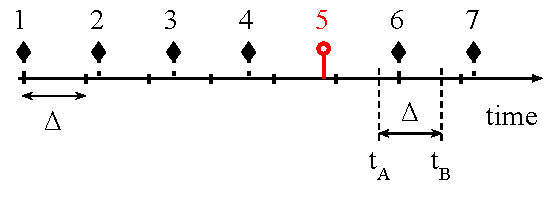
\includegraphics[width=0.4 \columnwidth,keepaspectratio]{figures/regular-adv-honest-queries.pdf}
    \caption{A series of successful honest (black solid diamonds) and adversarial (red hollow circles) queries
             regularly spaced apart more than $\delta$.}
    \label{fig.regular-adv-honest-queries}
\end{figure}

This scenario leads to the \emph{blocktree}\index{Blocktree} illustrated in Figure~\ref{fig.chain-fork}.
Worse yet, now some parties who detected that $5$ was broadcast late will accept $6$ as valid, whereas
the parties who received $5$ early will accept $7$ as valid. While we were hoping that the proof-of-work
construction would give us a single chain as a global source of truth, we have failed, and, again,
we have honest views in disagreement.

% todo: add the network timeline of parties 6 and 7 to illustrate how messages were received
\begin{figure}[h]
    \centering
    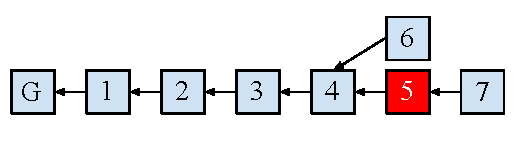
\includegraphics[width=0.4 \columnwidth,keepaspectratio]{figures/chain-fork.pdf}
    \caption{A block\emph{tree} instead of a block\emph{chain} arising out of the timeline
             of figure~\ref{fig.regular-adv-honest-queries}.}
    \label{fig.chain-fork}
\end{figure}

There is a disagreement about what is fresh and what is unfresh. We need to adopt a more
robust measure of time. Towards this, let us reinspect the chain structure we discovered
in the previous chapter.

Because the hash of a block cannot be predicted prior to the proof-of-work actually taking place
(otherwise proof-of-work would be solvable by a faster algorithm than exhaustive search),
the value
$s$ of the previd must be computed prior to the value $H(s \concat \overline{x} \concat \ctr)$.
In other words, the previd $s$ must already be known when mining for a new block that includes
$s$ as its previd. Blocks are mined in the order they appear. The pointers between blocks
in the chain are \emph{causality links}. They point backwards in time. The blockchain grows
forward in time and defines an \emph{arrow of time}\index{Arrow of Time}. When we observe a blockchain, we can
deduce that all of its blocks were mined one after the other in the order that we observe
them. In fact, if we have a blockchain consisting of a sequence of blocks, if we change
the payload $\overline{x}$ in an earlier block, this will cause the proof-of-work in that
same block and all subsequent blocks to become invalid: Changing the $\overline{x}$ of the
block will cause its own blockid to change and its proof-of-work to be invalidated. This, in
turn, requires changing the previd $s$ of the next block to maintain the chain structure,
causing \emph{its} proof-of-work to
be invalidated, and so on and so forth for every subsequent block on the chain, as
illustrated in Figure~\ref{fig.blockchain-invalidation}. To change
the contents of one block of the chain, the adversary would have to go back and redo all
the proof of work. Hence, the adversary cannot detach a block from its parent and append
it to a different parent to make it appear newer than it is.

\begin{figure}[h]
    \centering
    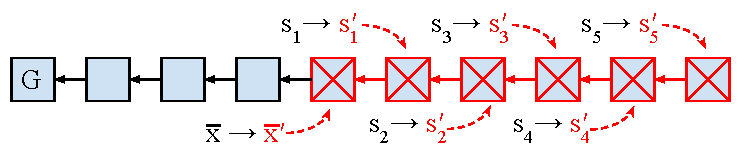
\includegraphics[width=0.7 \columnwidth,keepaspectratio]{figures/blockchain-invalidation.pdf}
    \caption{Changing just one small part of a block's content causes a cascading effect invalidating the proof-of-work of the whole chain inheriting from that block.}
    \label{fig.blockchain-invalidation}
\end{figure}

A longer blockchain takes more time to generate, whereas a shorter blockchain takes less time
to generate (we will prove this relationship between blockchains and time precisely in
Chapter~\ref{chapter:earnest3}). Therefore, we can use the \emph{length} of a blockchain
to estimate how much time it took to generate, and how fresh its tip is.

This allows a more objective comparison about which chain to adopt. Since a longer chain takes
more time to produce than a shorter chain, its tip is roughly the ``freshest''.
We now adopt the following rule for which chain to choose among multiple candidate
chains:

\begin{quote}\index{Longest Chain Rule}
    \textbf{Longest Chain Rule. }
    Among all chains on the network, adopt the \emph{longest} chain (the one with the most
    blocks) as your \emph{canonical chain}\index{Canonical Chain}. If there are multiple
    competing chains of the same length, choose any chain arbitrarily.
\end{quote}

Using this rule, a node doesn't have to stay online on the network all the time to observe
which block is fresh and which one isn't. Additionally, two honest nodes that have seen the
same network messages, regardless of the order in which they received them, agree on their
verdict of which chain is best.

We can now summarize the honest miner's rules, which every honest miner is constantly running:

\begin{enumerate}
  \item Maintain a local canonical chain $\mathcal{C}$.
  \item Keep mining on the canonical chain.
  \item If mining is successful, broadcast the new block to the network, and update the local canonical chain.
  \item If not, keep mining.
  \item In the meantime, when a new valid chain arrives on the network,
        check its length, and update the local canonical chain if the
        newly arriving chain is longer than the existing canonical chain.
\end{enumerate}

The most common situation is for the canonical chain to be replaced by a new chain
that extends the previous chain by one more block. However, sometimes a chain appears
that is longer but does not extend the previous chain. In this case, we say that
the chain \emph{reorgs} (reorganizes)~\index{Reorg} and certain blocks are \emph{rolled
back}.

Once a party has adopted a canonical chain, reporting a ledger of transactions
to implement the \emph{read} operation of a full node is straightforward and
is depicted in Algorithm~\ref{alg.read-naive}. Given a chain
$\chain = (B_0, B_1, \ldots, B_{n-1})$, the ledger reported by the honest
party when the \emph{read} functionality is invoked is the sequence of
transactions in the same order as they appear on the chain.
Here, we use the notation $B.\overline{x}$ to denote the $\overline{x}$ component
of block $B = s \conc \overline{x} \conc \ctr$.
First, the ledger is initialized to be the empty sequence $[\,]$. The algorithm
then traverses each block $B$ of chain $\chain$ in chronological order (while we
use the notation $B \in \chain$, remember that $\chain$ is an ordered sequence
and not a set). The transactions of the genesis block $B_0$ are appended to the ledger, in the same
order as they appear within the genesis block's transaction sequence $B_0.\overline{x}$
(which, again, is a sequence and not a set of transactions);
next, the transactions of the block following genesis are appended; and so on, until
the transactions of the tip are appended.

\import{./}{algorithms/alg.read-naive}

As you can judge by the name of this rule, this is a rule which we plan to
soon revise (in Chapter~\ref{chapter:virtues}).

\section{The Stochastic Nature of Work}

Despite adopting the Longest Chain Rule, the situation with successful queries
is far worse than we anticipated.
So far, we have presented successful queries as being
spaced apart \emph{exactly} $\frac{1}{pnq}$, but mining is a stochastic process which will have
irregularities. The value $\frac{1}{pnq}$ is just the \emph{expected} block generation time, but
sometimes successful queries will be spaced apart more closely and sometimes sparsely, as illustrated
in Figure~\ref{fig.stochastic-queries}. While we attempted to space queries reasonably apart, it can
just so happen that certain queries are successful in close proximity (less than $\Delta$ apart).
This means that, even without the presence of an adversary, the honest parties can happen to
mine blocktrees and be in disagreement.

\begin{figure}[h]
    \centering
    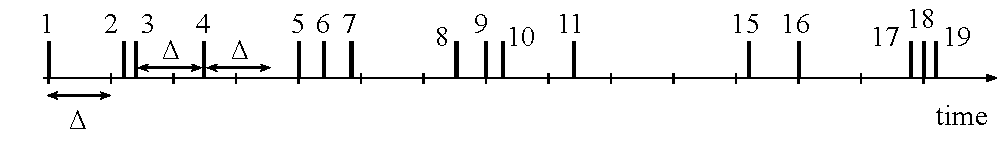
\includegraphics[width=0.8 \columnwidth,keepaspectratio]{figures/stochastic-queries.pdf}
    \caption{The stochastic nature of work makes honest successful queries irregular.}
    \label{fig.stochastic-queries}
\end{figure}

In Figure~\ref{fig.honest-chain-fork}, we illustrate a
blocktree that can arise out of the timeline of queries in Figure~\ref{fig.stochastic-queries}.
Even though \emph{all} successful queries were honest, the honest parties who used the longest
chain rule built a blocktree and not a single blockchain. At the end of the execution, the honest
parties are split between the canonical chains they have adopted: Some parties have adopted
the chain ending on block $17$, some have adopted the chain ending on block $18$, and some have
adopted the chain on block $19$, as their canonical chain. If these three blocks contain double
spends, the different honest parties could be reporting different ledgers. This happened even
though the adversary was not mining any blocks. This is a loss of safety.

Are we back to square one? Not quite. We'll soon see that, with a few last modifications to
our protocol, we can soon achieve security. We'll finish the protocol design in the next chapter,
and prove its security in Chapters~\ref{chapter:earnest1}-\ref{chapter:earnest3}. For the moment,
let us try to understand how the longest chain protocol works a little more precisely.

% TODO: change this blocktree so that some temporary fork is 2 blocks long
\begin{figure}[h]
    \centering
    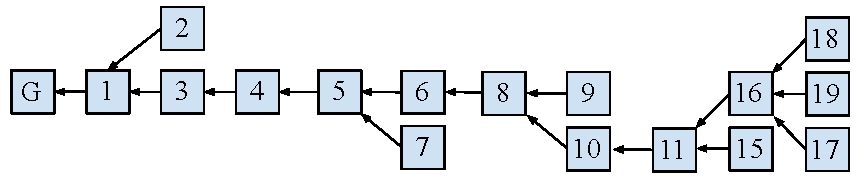
\includegraphics[width=0.8 \columnwidth,keepaspectratio]{figures/honest-chain-fork.pdf}
    \caption{A blocktree arising out of the timeline of honest-only queries of Figure~\ref{fig.stochastic-queries}.}
    \label{fig.honest-chain-fork}
\end{figure}

Let's go back to Figure~\ref{fig.honest-chain-fork}. In this picture, we notice that there
really is only one longest chain in the blocktree, except with some extra blocks here and
there. This longest chain begins from genesis and goes on until block $16$. Here and there
on the sidelines of the longest chain, we see a few blocks popping up such as block $2$
and block $7$. These smaller branches alongside the longest chain are called \emph{temporary
forks}\index{Temporary Fork} and can be one or more blocks long, but typically these
temporary forks will be quite short. We'll explore the reason for this in the next chapter.

Our chain's lifecycle begins at genesis, with every honest party mining on top of it.
When there is a single block mined by just one honest party, and that block makes it to
the doorstep of every other honest party before they've had the opportunity to mine their
own block, the chain grows for everyone. This is the usual case. In rare occassions, two
different honest parties will mine two different blocks at approximately the same time.
Because the one honest party has not received the block of the other honest party while
he is mining his own, both of these blocks will extend the same parent, so we will have a
temporary fork. We say that the chains of honest parties have diverged.
These two forks will now have the same height, and so the honest population
may be split among which one to adopt. If it so happens that the honest parties again
mine two different blocks at about the same time across the different forks, these temporary
forks will grow. However, as soon as there is a block mined on any of the
two temporary forks, and no other block is mined in close temporal proximity to it,
there will be one definitive longest chain, and every honest party will adopt it.
We say that the honest chains have converged again.

We notice that, in the optimistic setting where no adversary is mining, the honest parties
\emph{converge} on one chain whenever there is an honest successful query separated $\Delta$
from all other honest successful queries (it is also possible that honest parties converge
in other moments if they get lucky). Therefore, we call these moments in time \emph{convergence
opportunities}:

\begin{definition}[Convergence Opportunity (informal)]\index{Convergence Opportunity}
    An honest successful query is called a \emph{convergence opportunity} if it is $\Delta$
    separated in time from all other honest successful queries.
\end{definition}

Notice that the definition of a convergence opportunity only requires that an honest successful
query is separated from other \emph{honest} successful queries. It does not concern itself with
adversarial queries. It is possible that an adversary will cause a divergence even during a
convergence opportunity.

Convergence opportunities are events that are visible in \emph{God's eye} who has a full
and current global view of each and every party. The individual parties may not be able to tell
whether a successful query is also a convergence opportunity. The hope is that, even though honest
parties cannot detect convergence opportunities, these will still happen behind the scenes
and will lead to convergence. While this convergence will take place often, the honest
parties will not be aware of whether convergence has occurred, but this will not cause
any issue.

\section{The Honest Majority Assumption}\index{Honest Majority Assumption}

% TODO: why is the honest majority assumption a "reasonable" assumption?

Even though we used the longest chain rule to ensure that blocks from the long past are not
retroactively revived, an adversary with large mining power compared to the honest parties can
still mine in secret. Look at Figure~\ref{fig.adversarial-majority}. Here, the honest parties
mine sequentially on top of block $1$ and produce block $2$ and its descendants.
The adversary independently mines on top of block $1$ and produces $2'$ and its descendants,
which the adversary does not broadcast to the network yet. When the adversary has accumulated
a bunch of more blocks than the honest party, he broadcasts the whole chain to the network.
The honest parties adopt the newly broadcasted adversarial chain, abandoning their own.

\begin{figure}[h]
    \centering
    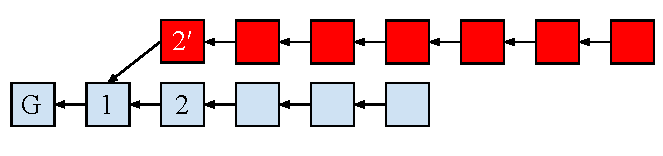
\includegraphics[width=0.6 \columnwidth,keepaspectratio]{figures/adversarial-majority.pdf}
    \caption{An adversary with dishonest majority (top red chain) can outpace the honest parties (bottom
             blue chain).}
    \label{fig.adversarial-majority}
\end{figure}

This situation is pretty bad. It causes a \emph{loss of safety}, as some of the honest parties have
switched from their ledgers to the adversary's ledger, causing disagreement. It also causes a
\emph{loss of liveness}, because the adversary may choose not to include any honest transactions.
However, if the adversary
only has a minority of mining power, even though these attacks can start small, they cannot grow
for much longer, as the adversary will be left behind in the dust by the honest parties who will
be mining more quickly.
We'll explore these attacks much more deeply in Chapter~\ref{chapter:attacks},
and we'll formalize them in Chapter~\ref{chapter:earnest1}. However, it should already be clear
that we must require that the adversary controls only a minority of the compute of the network.
We will call this the \emph{honest majority assumption}.

\begin{definition}[Honest Majority Assumption]
  The \emph{honest majority assumption} mandates that the adversary controls less compute than
  the honest parties:

  \[
    t < n - t
  \]
\end{definition}

Using the honest majority assumption, and with a small modification to the way we read ledgers,
in the next chapter we will intuitively argue that our protocol is now secure.

\section{Coinbase Transactions}

Now that we have completed the design of our longest chain protocol, we have finally solved the
problem of how money is \emph{transferred} in a publicly verifiable and decentralized manner.
However, we never tackled the problem of how money is \emph{created} in a decentralized manner.
If there is no central authority to issue money, how can we create new money, and who receives
any new money that is created? With the invention of blocks, there is a natural choice for this.
Since blocks are generated in regular intervals, we can use the block to inject the money supply
with new money in a manner that maintains controlled scarcity.
This is where the \emph{coinbase} transaction comes into play.
Recall that a coinbase transaction has no inputs and a single output with a certain value coming
out of it, as illustrated in Figure~\ref{fig.coinbase}.
It is the only type of transaction that does not respect the Conservation Law.
Our rule says that every block
must have \emph{at most one} coinbase transaction, and that transaction must appear \emph{first} in
the list of transactions of the block, if at all (different blockchain systems may have slightly
different details on what rules they enforce on the syntax of coinbase transactions).
The public key in the output of the coinbase transaction is freely chosen by the miner.
Naturally, because this is free money, the miner will typically make that public key
be their own, so that they can reap the benefits of mining.

\begin{figure}[h]
    \centering
    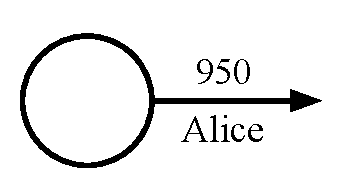
\includegraphics[width=0.23 \columnwidth,keepaspectratio]{figures/coinbase.pdf}
    \caption{A coinbase transaction paying Alice the amount of 950 units. The coinbase has no inputs and a single output.}
    \label{fig.coinbase}
\end{figure}

We now need to make a decision about how much money can appear in the output of the coinbase
transaction of each block. The value on the coinbase transaction has two parts: A block \emph{reward}
and the \emph{transaction fees}.

The \emph{block reward}\index{Block Reward} $f_r$ corresponds
to money that is newly created. This money comes out of thin air, and is injected into the system
without coming from anywhere. It is how new money is created. The block reward must follow an
algorithmic, prespecified rule that is hard-coded into the system. One simple way is to set a fixed
amount to be the limit of the block reward, and ensure every full node has this amount hard-coded
into its source code. For example, we can set the block reward to simply be the constant $f_r = 50$ units.
During the validation of a coinbase transaction, each client checks that this
amount is respected. In case the coinbase transaction deviates from this rule, the coinbase transaction
is considered invalid, and so is the block it is contained in. The decision on how the block reward
is algorithmically determined is called the \emph{macroeconomic policy} of the chain. We'll have
more to say about this in Chapter~\ref{chapter:economics}. Let's observe what exactly is happening
with this construction. Instead of having an authority decide how much new money is created, this
decision is fixed upfront and known to everyone beforehand. And instead of having an authority
receive the newly created money and decide what to do with it, we \emph{randomly} allocate this
new money to the lucky node who happened to be the successful miner of the block.

The second part of the value of the coinbase transaction output consists of the \emph{transaction fees}\index{Fees}.
Revisiting the Weak Conservation Law, remember that it's possible that some transactions can have
more input value than output value, because we only demanded that

\[
    \sum_{i \in \tx\textsf{.ins}} i.v \geq \sum_{o \in \tx\textsf{.outs}} o.v\,.
\]

If this inequality is strict, then there is more input value than output value, as illustrated
in Figure~\ref{fig.fee}. That difference in value
is not lost, but the miner is allowed to reclaim it as part of their coinbase value.

\begin{figure}[h]
    \centering
    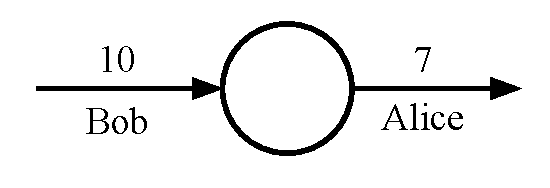
\includegraphics[width=0.4 \columnwidth,keepaspectratio]{figures/fee.pdf}
    \caption{A transaction with an input of $10$ and an output of $7$ pays a fee of $3$ units that
             go to the coinbase output.}
    \label{fig.fee}
\end{figure}

Overall, the coinbase transaction is allowed to include up to a value which is the sum of
the block reward plus the transaction fees of all the transactions. The total amount of fees
incurred in a block $B$ will be

\[
    f_f(B) = \sum_{\substack{\tx \in B\textsf{.}\overline{x}\\\tx \text{ non-coinbase}}}{\sum_{i \in \tx\textsf{.ins}} i.v - \sum_{o \in \tx\textsf{.outs}} o.v}\,.
\]

The coinbase output value is allowed to be up to the total $f_t = f_r + f_f(B)$ which includes both
the reward and the fees. Typically, the miner will claim the maximum allowed value in the coinbase.
In case the miner chooses not to claim the full value, that money is \emph{burned} and does not belong
to anyone.

To verify a coinbase transaction, we follow these steps:
\begin{enumerate}
    \item Check that is is the only one in that block.
    \item Check that it is the first transaction in the block.
    \item Check that it has no input and exactly one output.
    \item Check that its output has a value which is less than or equal to the sum of the block reward and the difference between the input and output amounts of all \emph{other} transactions in the block.
    \item Check that the coinbase is not spent in the same block.
\end{enumerate}

The last condition is known as the coinbase \emph{maturation}\index{Coinbase Maturation} condition,
and sometimes a longer waiting time than one block is required.

One more technical detail is required in the data that is included in the coinbase transaction.
Because the miner in two different blocks can be the same, and the value $f_t$ in two different
blocks may also be the same, all the data of two different coinbase transactions can be identical.
If we didn't take any action to prevent this, their $\txid$ would be identical as well.
However, we would still like to distinguish the two different coinbase transactions of different
blocks, so that they can be spent independently. It is therefore important to include some extra
metadata to distinguish one coinbase transaction from another. One such piece of metadata that
can be included is the block height of the block the coinbase transaction is included in.

With coinbase and regular transactions, we've concluded both the publicly verifiable \emph{creation}
and \emph{transfer} of money in a way that respects scarcity, completing our monetary design.

\section{Block Validation}

So far, we described how blocks are mined, but we have not given the block validation algorithm.
This algorithm is straightforward and consists of the following steps. Whenever an incoming
block $B = s \conc \overline{x} \conc \ctr$ arrives:

\begin{enumerate}
    \item Validate the proof-of-work $H(B) \leq T$.
    \item Use $s$ to locate its parent block and ensure it is valid recursively.
    \item Validate the transactions $\overline{x}$.
\end{enumerate}

To avoid spam, only valid blocks are gossiped by honest nodes. As it is moderately difficult to
create proof-of-work, this is validated first to avoid spam attacks. In case $s$ points to a block
that is not known to the node, this is downloaded and validated recursively. Similarly if
$\overline{x}$ refers to any transactions that are unknown, these are downloaded from the network
to validate the block.

The validation of transactions
$\overline{x}$ in a block works as follows. For each block $B$, we remember a UTXO set which we
associate with the state $\st(B)$ of the world \emph{after} the particular block has been adopted.
We also define a \emph{genesis state}\index{Genesis State} $\st_0$, the state of the world \emph{before}
any transaction ever
took place. The genesis state, which is where the UTXO set begins its lifetime, is defined to be the
empty set.

To validate the transactions in a block $B = s \conc \overline{x} \conc \ctr$, we take the state
$\st_{B'}$ associated with
its parent block $B'$ whose blockid is $s = H(B')$, or $\st_0$ if $B = \mathcal{G}$.
We then attempt to apply each of the transactions in the block, in the order
they are defined in $\overline{x}$, updating the UTXO set as we go along by consuming
and producing elements in the set, and validating
every transaction along the way, in the manner we already discussed in Chapter~\ref{chapter:transaction}.
If at any point the transaction validation fails, the whole block is rejected,
even if just one transaction was invalid. If all transaction validations succeeded,
we assign the state $\st_B$ after our block to be the UTXO set we arrived at after
this process is completed. This is illustrated in Figure~\ref{fig.block-tx-validation}.
% This figure number shows up unrendered for me
In this example, $B.\overline{x} = (\tx_1, \tx_2, \tx_3, \tx_4)$.

\begin{figure}[h]
    \centering
    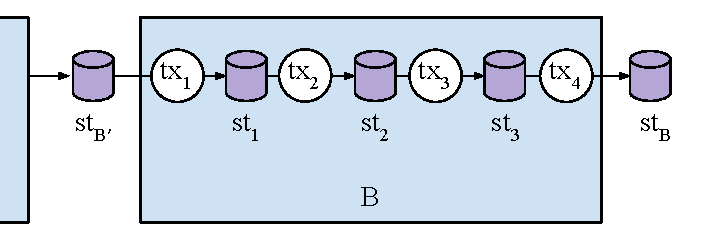
\includegraphics[width=0.7 \columnwidth,keepaspectratio]{figures/block-tx-validation.pdf}
    \caption{Validating the $\overline{x}$ part of block $B$. The intermediate states
             are shown as purple cylinders. The state $\st_{B'}$ comes from a block
             which has already been validated (shown partially on the left).}
    \label{fig.fee}
\end{figure}

While we will sometimes say that \emph{chains} are exchanged on the network, it is really
\emph{blocks} that are sent over the network. Due to the fact that each block contains
a reference to its parent, a block uniquely identifies the chain of which it is a tip.
When a party wishes to send a chain to another party, it is sufficient that the tip is
sent over. The other party can then request the ancestor blocks if he doesn't already
have them.
In practical protocols, sometimes these requests for objects are bundled
together in batches to improve communication complexity. For example, all the transactions
of one block can be downloaded in one go instead of requesting each of them independently.
Validating a chain equates to validating its tip, as this requires validating
the parent block recursively. The genesis block is hard-coded into every full node and is
considered valid by definition. This is where the recursion stops.

\section{Maintaining the Mempool}

As we have already discussed in the previous chapter, each node maintains a \emph{mempool}
with transactions in limbo, waiting to be confirmed into a block. A \emph{mempool state}\index{Mempool State}
is maintained pertaining to the current mempool. This state is where newly arriving unconfirmed
transactions are checked against for validity. When a new transaction arrives from the network,
after it is validated, this mempool state is updated to reflect the consumption and creation
of elements in the UTXO set. If the miner is able to
get a block, the mempool transactions make it into the block and the mempool is emptied.
At this point, the mempool state becomes equal to the state of the newly mined block.
However, if a \emph{different} party successfully mines a block, we have to be a little
more careful about updating our mempool and the mempool state, as our mempool may not exactly
match the transactions that were received in the newly arriving block.

Consider the case where a party $P_1$ has some chain $\chain$ and party $P_2$ mines a new
block $B$ on top of $\chain$. As usual, the block $B$ is validated with respect to the state
$\st(\chain)$ of $\chain[-1]$. After validation, we have calculated the state $\st(B)$ of $B$.
Now, $P_1$ calculates the \emph{new} mempool $\overline{x}'$ as follows.
He first sets the mempool state to be equal to the state $\st(B)$ of the latest block.
He looks at the transactions $\overline{x}$ in his \emph{old} mempool and processes them
one by one. He attempts to apply each of these transactions $\tx \in \overline{x}$ in the
order that they appeared in his old mempool on top of $\st(B)$, updating the mempool state every time
a transaction is successfully applied. If a transaction from the old mempool
cannot be applied, that transaction is thrown away and the mempool state remains unaffected.
The transactions that are applied successfully
make it to the new mempool. This process is like pretending that each of the old mempool transactions
appeared on the network in order after block $B$ was processed. If block $B$ contains a transaction
that was in the old mempool (which will typically be the case), then this transaction has already
been applied in $\st(B)$, and so will not make it into the new mempool, because it is spending already
spent outputs. If block $B$ contains a transaction that is conflicting with a transaction
in the old mempool, then the transaction in the old mempool will also be thrown out, because it
is conflicting with the transaction in $B$ that has already been applied to $\st(B)$.
As such, if two mutually double spending transactions appear in a block and in the mempool,
the transaction in the block takes precedence.

The situation becomes slightly more complicated when there is a reorg. In that case, the
state is rolled back to after the latest common ancestor between the old canonical chain and
the new reorged chain, and state transitions are applied from that point onwards. As for the
new mempool, it is reconstructed by attempting to apply first all the transactions in the
abandoned fork, and then the transactions in the old mempool.

This algorithm will be made clearer with an example. Consider the situation illustrated in
Figure~\ref{fig.chain-state-validation}, and suppose our party has adopted the chain
whose tip is $B'_2$ (bottom) and has a mempool of $\overline{x}'$. Suddenly, block $B_3$
arrives. The party downloads the chunk $(B_1, B_2, B_3)$ and validates it. As before,
this validation begins by looking at the state of the latest common ancestor $B$.
This has the effect that all the transactions in $B_1'$ and $B_2'$ are undone
prior to applying the transactions in $B_1$.
First, the transactions in $B_1$ are applied and $\st(B_1)$ is calculated. Then
$B_2$ is applied and $\st(B_2)$ is calculated. Lastly, $B_3$ is applied and $\st(B_3)$
is calculated. If at any point a transaction cannot be applied, the whole block containing
it is rejected.

Now suppose that the newly arriving chain was valid. Since $B_3$ has a higher height than $B'_2$,
the chain ending in
$B_3$ is adopted by the longest chain rule.
At this time, the party wants to compute his new mempool $\overline{x}$.
This is done as follows. The party begins by setting the mempool state to $\st(B_3)$.
First, all the transactions $B_1'.\overline{x}$ are trialed for placement into the new
mempool in the same order they appear within $B_1'.\overline{x}$. Similarly, the
transactions in $B_2'.\overline{x}$ are trialed for placement into the new mempool.
Lastly, the transactions in the old mempool $\overline{x}'$ are trialed for placement
into $\overline{x}$. Every time a transaction can be applied successfully, it is
added to the new mempool, and the mempool state is updated. In case a transaction
is unapplicable, the transaction is thrown away and the mempool state remains unaffected.

\begin{figure}[h]
    \centering
    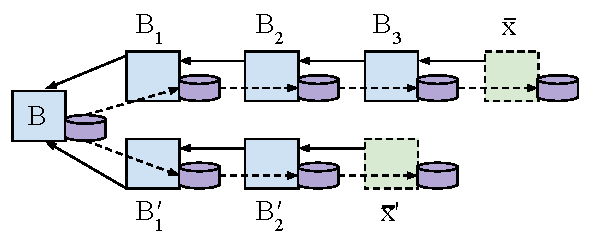
\includegraphics[width=0.7 \columnwidth,keepaspectratio]{figures/chain-state-validation.pdf}
    \caption{The state and mempool calculation in the case of a reorg. Ancestry relations
             are shown in solid arrows, whereas state updates are shown in dashed arrows.
             Blocks are depicted as blue solid bloxes; states are depicted as purple cylinders;
             mempools are depicted as dashed green boxes.}
    \label{fig.chain-state-validation}
\end{figure}

This has the effect that, after a reorg, between any transactions that have a double spend in both
the abandoned fork and the newly adopted chain, the transaction in the new
chain takes precedence, whereas the double spend within the abandoned fork is also abandoned
(and is not even placed in the new mempool). This illustrates why reorgs can be dangerous:
Money that is already considered \emph{confirmed} can be rolled back, and a double spend can later
become confirmed in its stead.

% TODO: reorg algorithm in pseudocode

\section{Problems}

TBD

\section{Further Reading}

TBD
